\documentclass[12pt]{article}
\usepackage[margin=2.5cm]{geometry}

\usepackage[english]{babel}
\usepackage[utf8]{inputenc}
\usepackage[T1]{fontenc}
\usepackage{amsmath}
\usepackage{esint}
\usepackage{amssymb}
\usepackage{csquotes}
\usepackage{mathtools, graphicx, hyperref, url, svg}
\usepackage{caption}
\usepackage{subcaption}
\usepackage{systeme}
\usepackage{esvect}
\usepackage{amsmath,systeme}
\usepackage{multirow}
\makeatletter
\renewcommand*\env@matrix[1][*\c@MaxMatrixCols c]{%
  \hskip -\arraycolsep
  \let\@ifnextchar\new@ifnextchar
  \array{#1}}
\makeatother

\usepackage{biblatex} %Imports biblatex package
\addbibresource{references.bib}


% För att färga tabellkoloumner
\usepackage{colortbl}

\newcommand{\mc}[2]{\multicolumn{#1}{c}{#2}}
\definecolor{LightCyan}{rgb}{0.88,1,1}

%\newcolumntype{a}{>{\columncolor{Gray}}c}
%\newcolumntype{b}{>{\columncolor{white}}c}

%% För att skriva koden
\usepackage{listings}
\usepackage{color}
\usepackage{inconsolata}

\definecolor{codegreen}{rgb}{0,0.6,0}
\definecolor{codegray}{rgb}{0.5,0.5,0.5}
\definecolor{codepurple}{rgb}{0.58,0,0.82}
\definecolor{backcolour}{rgb}{0.95,0.95,0.92}


\lstset{frame=tb,
  language=Python,
  aboveskip=3mm,
  belowskip=3mm,
  showstringspaces=false,
  columns=flexible,
  basicstyle={\small\ttfamily},
  numbers=none,
  backgroundcolor=\color{backcolour},
  numberstyle=\tiny\color{codegray},
  keywordstyle=\color{magenta},
  commentstyle=\color{codegreen},
  stringstyle=\color{codepurple},
  breaklines=true,
  breakatwhitespace=true,
  tabsize=3
}

\lstset{literate=
  {á}{{\'a}}1 {é}{{\'e}}1 {í}{{\'i}}1 {ó}{{\'o}}1 {ú}{{\'u}}1
  {Á}{{\'A}}1 {É}{{\'E}}1 {Í}{{\'I}}1 {Ó}{{\'O}}1 {Ú}{{\'U}}1
  {à}{{\`a}}1 {è}{{\`e}}1 {ì}{{\`i}}1 {ò}{{\`o}}1 {ù}{{\`u}}1
  {À}{{\`A}}1 {È}{{\'E}}1 {Ì}{{\`I}}1 {Ò}{{\`O}}1 {Ù}{{\`U}}1
  {ä}{{\"a}}1 {ë}{{\"e}}1 {ï}{{\"i}}1 {ö}{{\"o}}1 {ü}{{\"u}}1
  {Ä}{{\"A}}1 {Ë}{{\"E}}1 {Ï}{{\"I}}1 {Ö}{{\"O}}1 {Ü}{{\"U}}1
  {â}{{\^a}}1 {ê}{{\^e}}1 {î}{{\^i}}1 {ô}{{\^o}}1 {û}{{\^u}}1
  {Â}{{\^A}}1 {Ê}{{\^E}}1 {Î}{{\^I}}1 {Ô}{{\^O}}1 {Û}{{\^U}}1
  {œ}{{\oe}}1 {Œ}{{\OE}}1 {æ}{{\ae}}1 {Æ}{{\AE}}1 {ß}{{\ss}}1
  {ç}{{\c c}}1 {Ç}{{\c C}}1 {ø}{{\o}}1 {å}{{\r a}}1 {Å}{{\r A}}1
  {€}{{\EUR}}1 {£}{{\pounds}}1
}

\setlength{\parskip}{1em} % Lämna en blankrad
\setlength{\parindent}{0em} % Indentera inte nya stycken

%%% TITEL %%%

\title{Exercise 4  - Classification}
\author{\textit{Computer Assisted Image Analysis 1  - 1TD396}  \vspace{1cm} \\
         Jennifer Andersson, David Björk \& Tove Gunnarsson \vspace{0.7cm}\\
        }
\date{\today}

%%% DOKUMENTET %%%
\begin{document}
\maketitle

\begin{figure}[b]
  \centering
  \includegraphics[width = 3cm]{images/UU_logo.pdf}
\end{figure}
\thispagestyle{empty}

\clearpage
%\tableofcontents

\newpage
%%%%%%%%%%%%%%%%%%%%%%%%% INTRODUCTION %%%%%%%%%%%%%%%%%%%%%%%%%%%%%%
\section{Classification Basics}


\textbf{\emph{Question 1.}}
% Are the two classes possible to separate by using either the x or y coordinate as a single feature? 
% Explain why or why not.

\begin{figure}[htbp!]
  \centering
  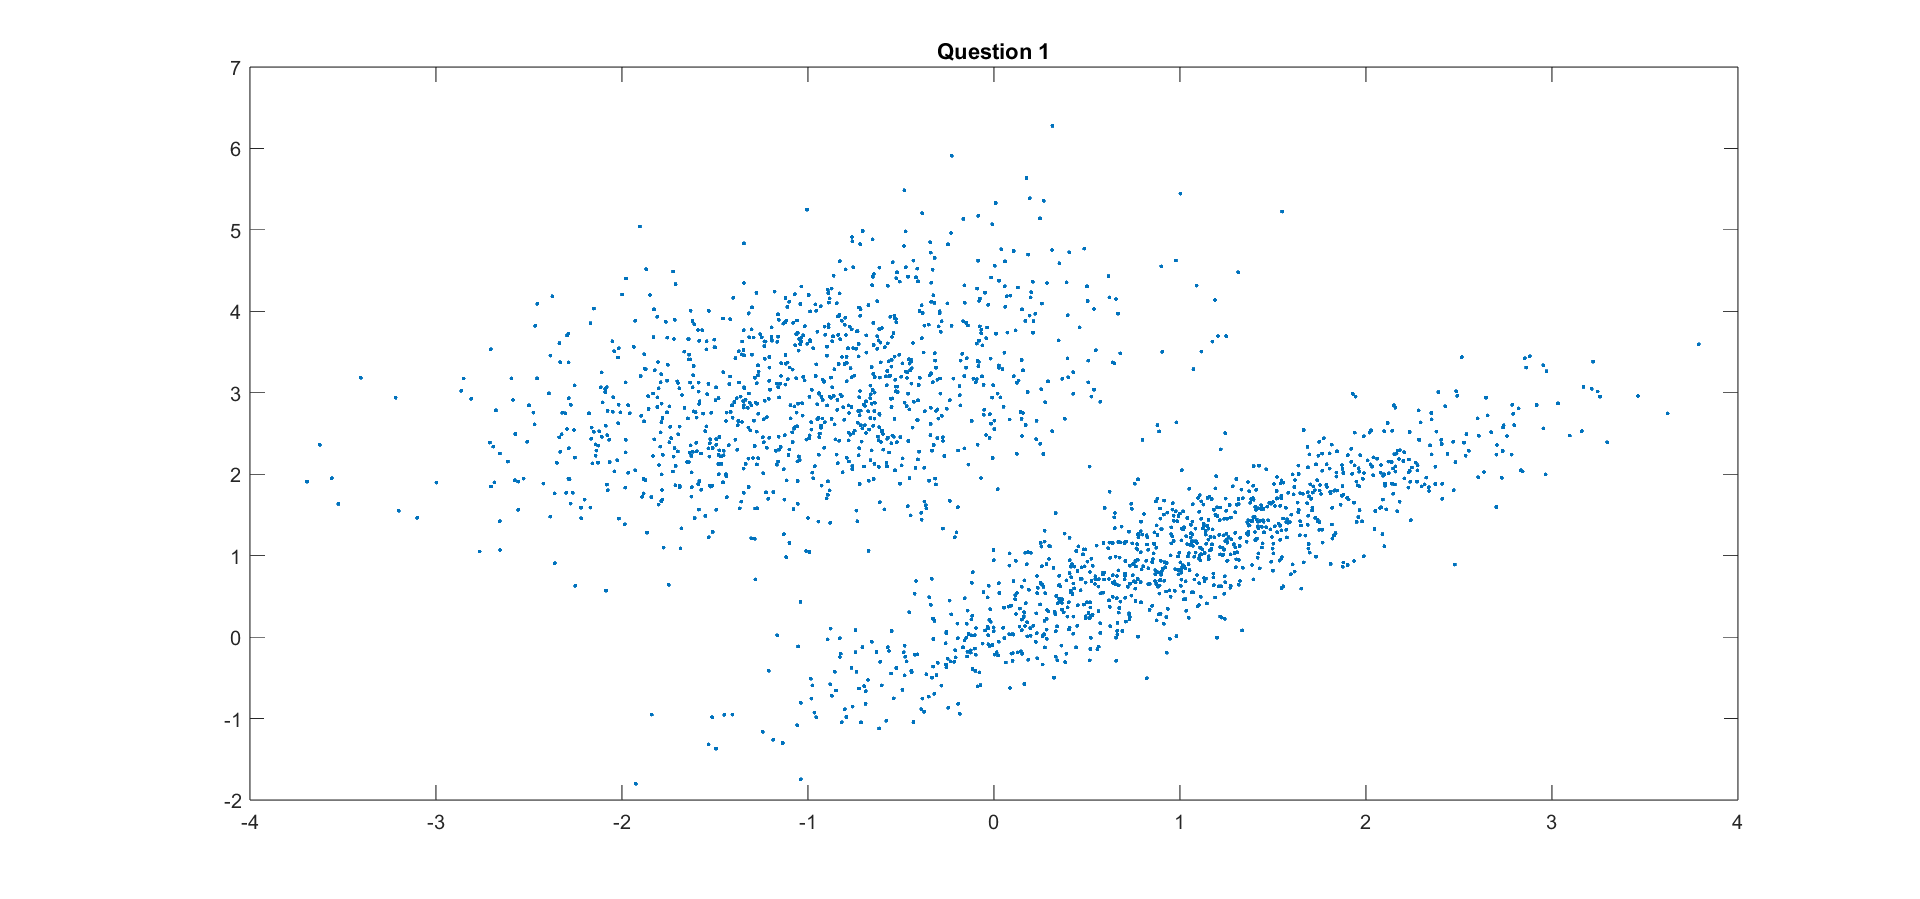
\includegraphics[width = 15cm]{images/Q1.png}
  \caption{Plot of the given data of two classes}
  \label{fig:Q1}
\end{figure}

As illustrated in Figure \ref{fig:Q1}, the dataset comprises two distinct classes that can be separated by a straight line. However, since the separating line is neither horizontal nor vertical, it is evident that a single feature alone is insufficient to achieve this separation. Consequently, both coordinates are required to effectively distinguish between the two classes.

\textbf{\emph{Question 2.}}
% Does multiple thresholding give a successful classification of the three classes?
% Explain why or why not
Multiple thresholds values were tried, where the best preformance was obtained with two threshold values at 92 and 137 as illustrated in the histogram in figure \ref{fig:Q2_hist}. The classification successfully classified the background, but failed to classify the ring against the hand, see figure \ref{fig:Q2_im}. This was due to the similiar color of the objects and as viewed in the histogram,  there is no siginiciant distinct threshold between the regions, since there exist some fluctiantions inbetween them. 

\begin{figure}[htbp!]
  \begin{subfigure}[b]{0.5\textwidth}
       \centering
       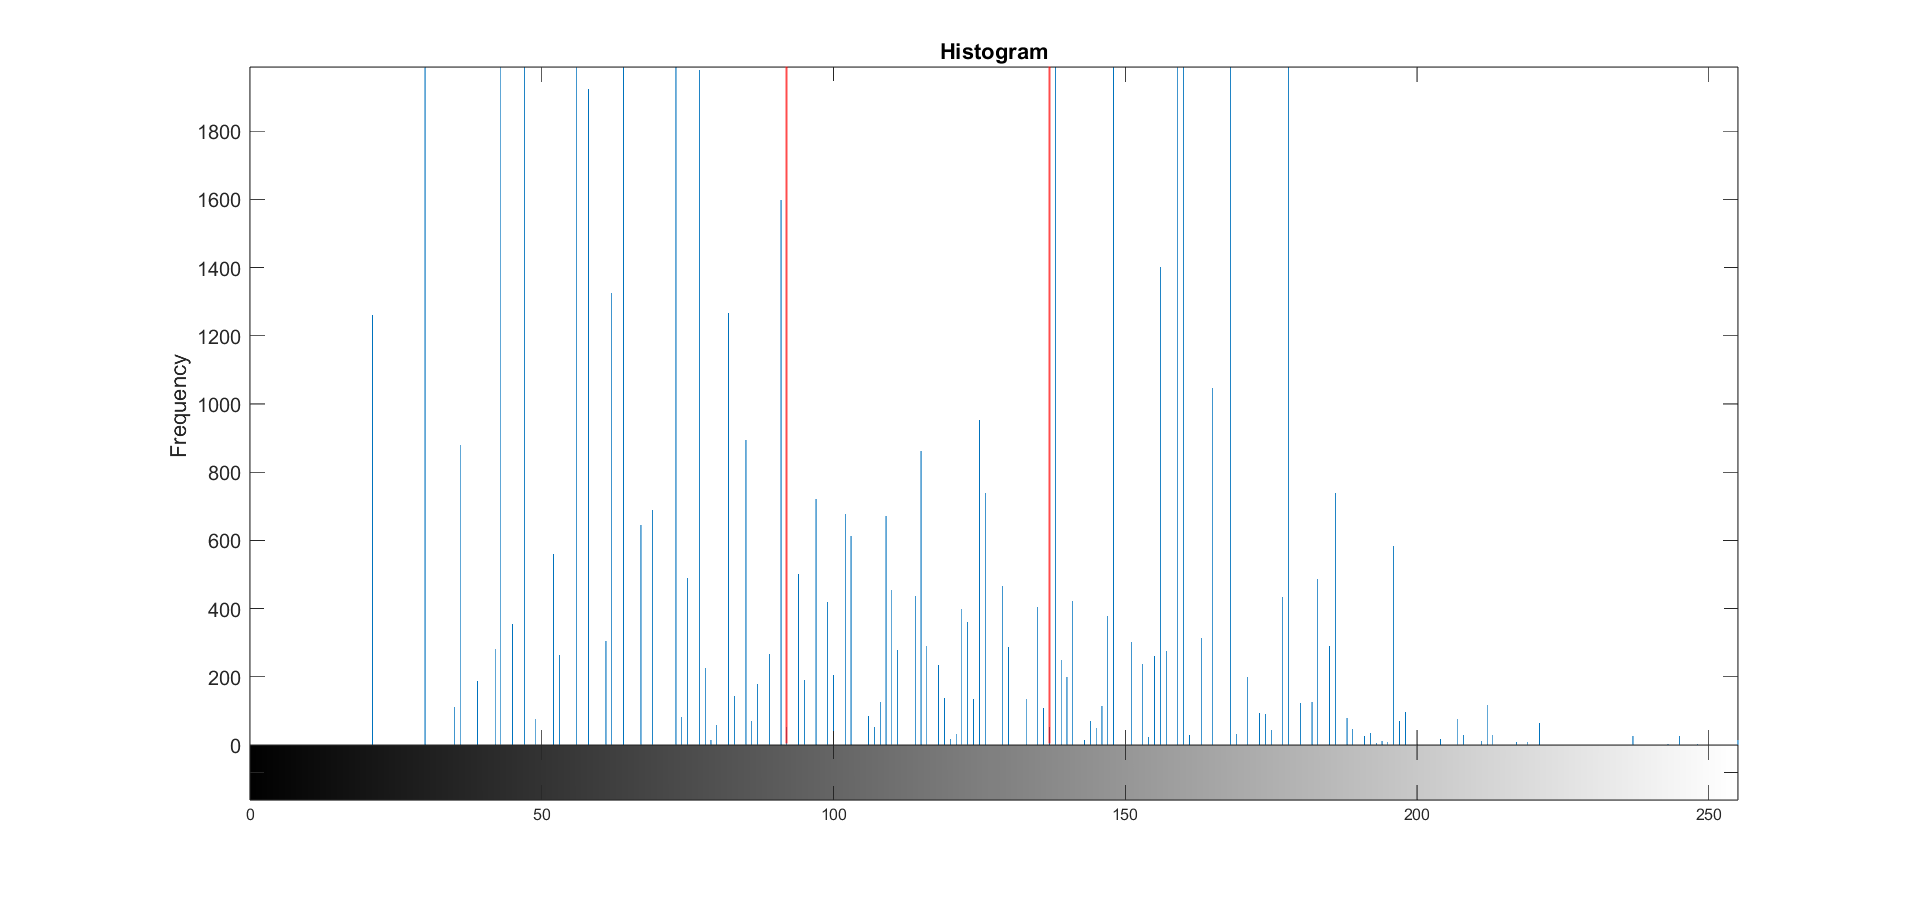
\includegraphics[width=0.9\linewidth]{images/Q2_hist.png}
       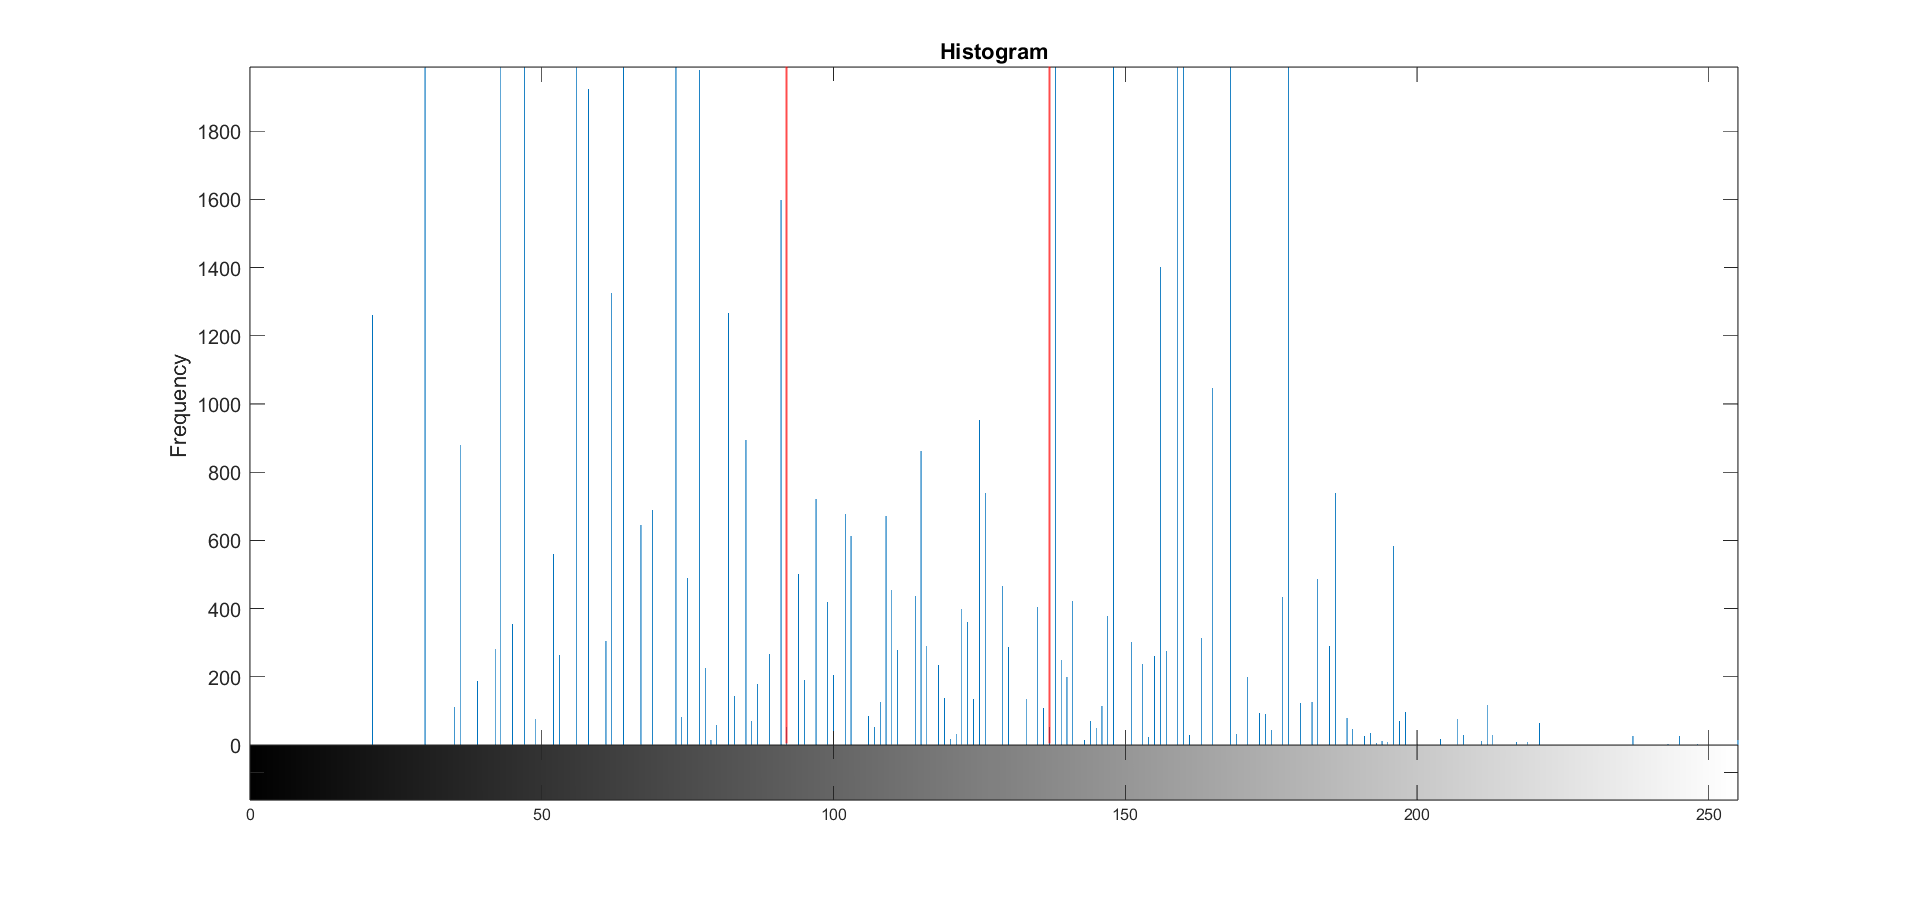
\includegraphics[width=0.9\linewidth]{images/Q2_hist.png}
       \caption{Histogram of the black and white image.}
       \label{fig:Q2_hist}
   \end{subfigure}
   \hfill
   \begin{subfigure}[b]{0.5\textwidth}
       \centering
       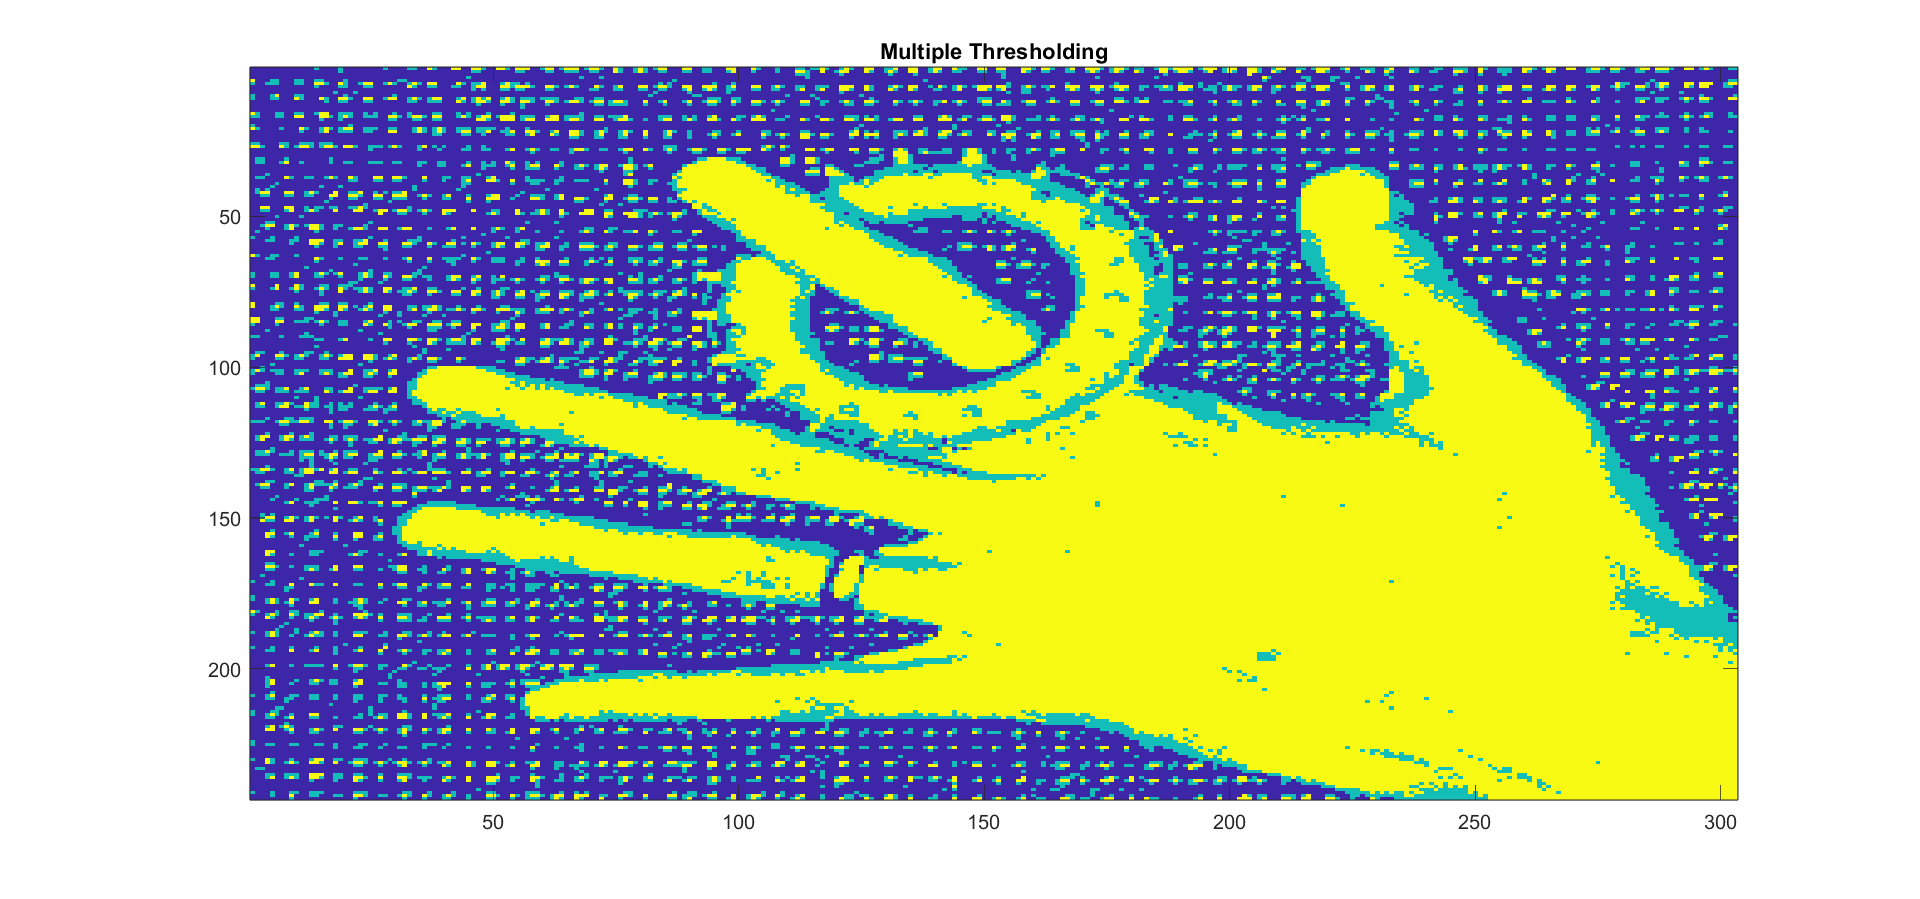
\includegraphics[width=0.9\linewidth]{images/Q2.png}
       \caption{Threshold classiciation of the grayscale image}
       \label{fig:Q2_im}
   \end{subfigure}
      \caption{Mulitple thresholding and its corresponding result of an grayscale image.}
      \label{fig:Q2}
\end{figure}


\textbf{\emph{Question 3.}}
% MATLAB’s classify function uses Linear Discriminant Analysis (LDA) as default.
% What assumptions are made on the data by an LDA classifier? 
% Also, what makes a classifier linear?
Linear Discriminant Analysis (LDA) is a classification technique that operates under the assumption that the features within each class are drawn from a Gaussian (normal) distribution and that all classes share a common covariance matrix. This shared covariance matrix ensures that the decision boundaries between classes are linear, which is a defining characteristic of the classifier. Specifically, the decision boundary is represented as a linear function of the input features, making LDA particularly effective for problems where this assumption holds true.

\textbf{\emph{Question 4.}}
% Have the results improved using classification compared to thresholding? Is the classification more successful in the case with the grayscale image or single bands? Explain.
% Does it improve the classification to incorporate pairs of bands or the full RGB information? Discuss. 
% Show your results from grayscale classification, one pair of features and full RGB classification

When comparing the performance of multiple thresholding and classification on the grayscale image, the classification method provided a more distinct separation of the background and demonstrated slightly improved object classification. However, the classification method was not entirely successful due to inconsistencies in the classification of colors within the objects themselves. The results of this analysis are presented in Figure \ref{fig:Q4_bw}.
\begin{figure}[htbp!]
  \centering
  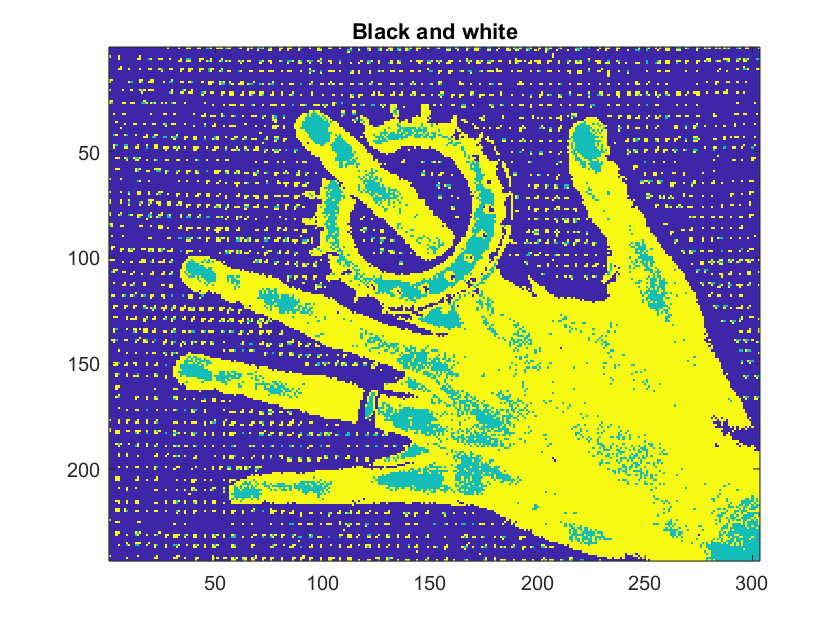
\includegraphics[width = 15cm]{images/Q4_bw.png}
  \caption{Result of classification of the grayscale image}
  \label{fig:Q4_bw}
\end{figure}
For the classification of individual bands of the image, the performance varied depending on the band used. As shown in Figure \ref{fig:Q4_1}, the green band produced the most accurate results, with the objects being the most clearly distinguished. In contrast, the red band failed to adequately classify the objects, while the blue band struggled to differentiate the hand from the background.
\begin{figure}[htbp!]
  \centering
  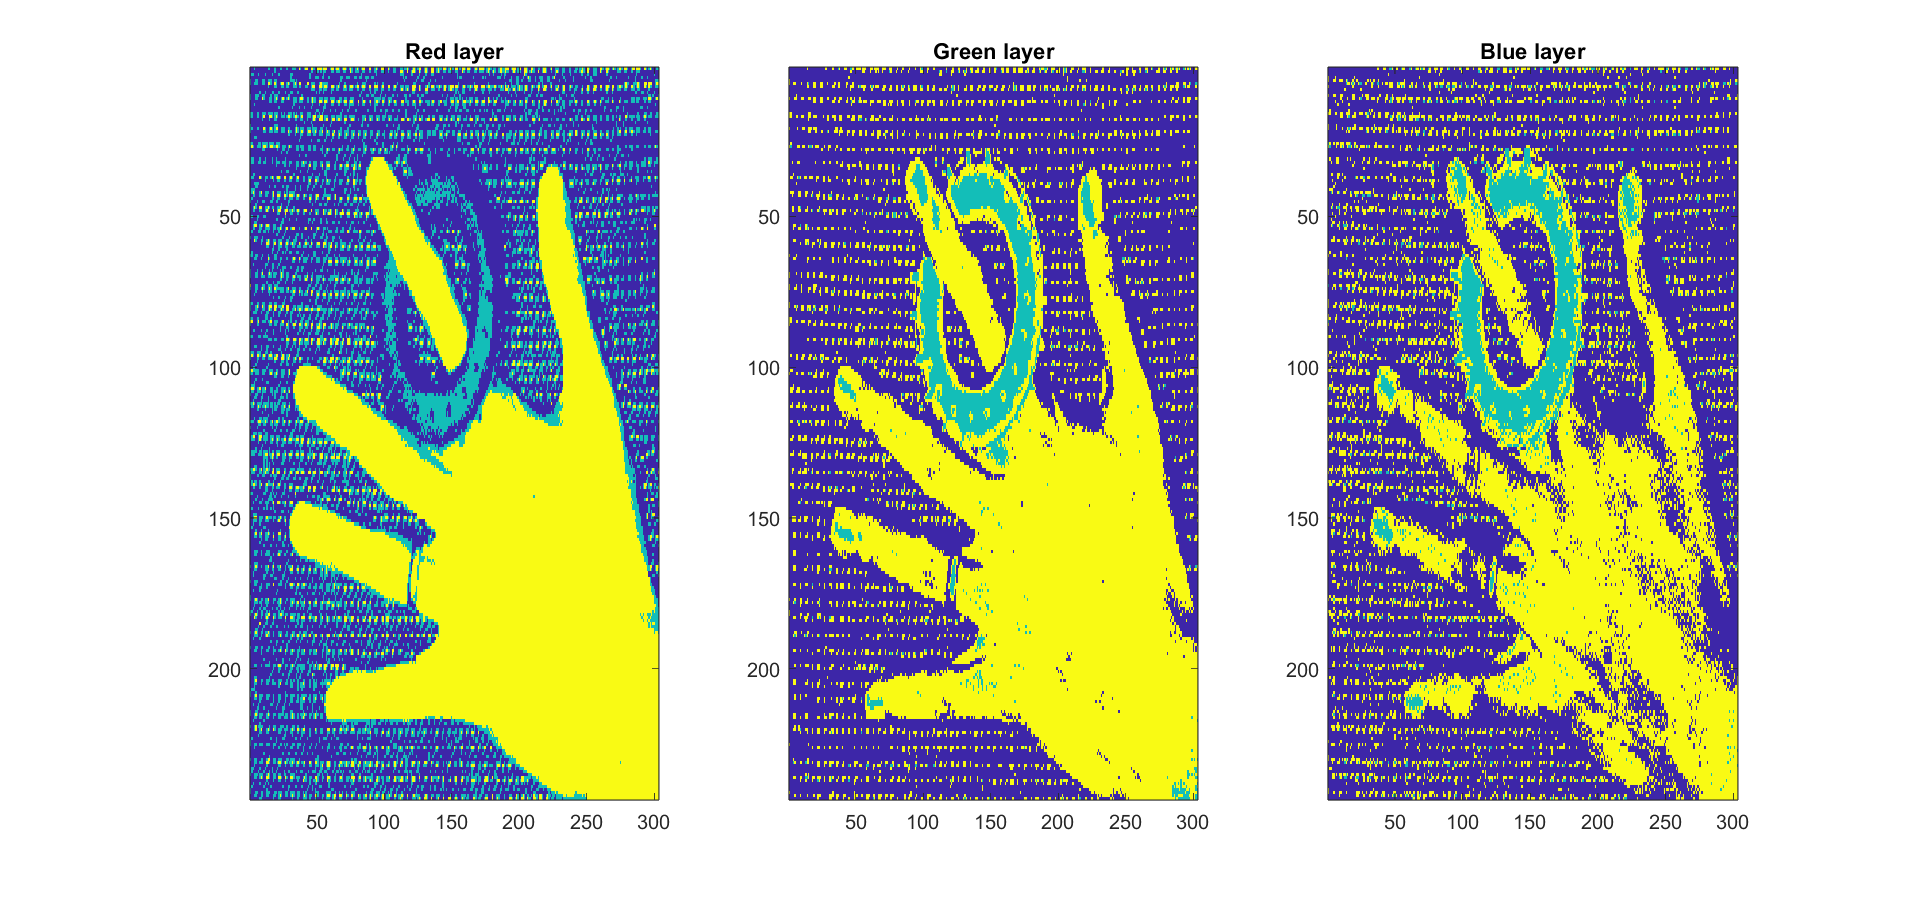
\includegraphics[width =\textwidth]{images/Q4_1b.png}
  \caption{Result of classification of single bands of the image}
  \label{fig:Q4_1}
\end{figure}
When pairs of bands were combined, the classification performance improved significantly, as illustrated in Figure \ref{fig:Q4_2}. Both the 'Red and Green' and 'Red and Blue' combinations successfully classified the objects and background with minimal noise. The 'Green and Blue' pair, however, yielded slightly less accurate results, with more noise present in the classification.
\begin{figure}[htbp!]
  \centering
  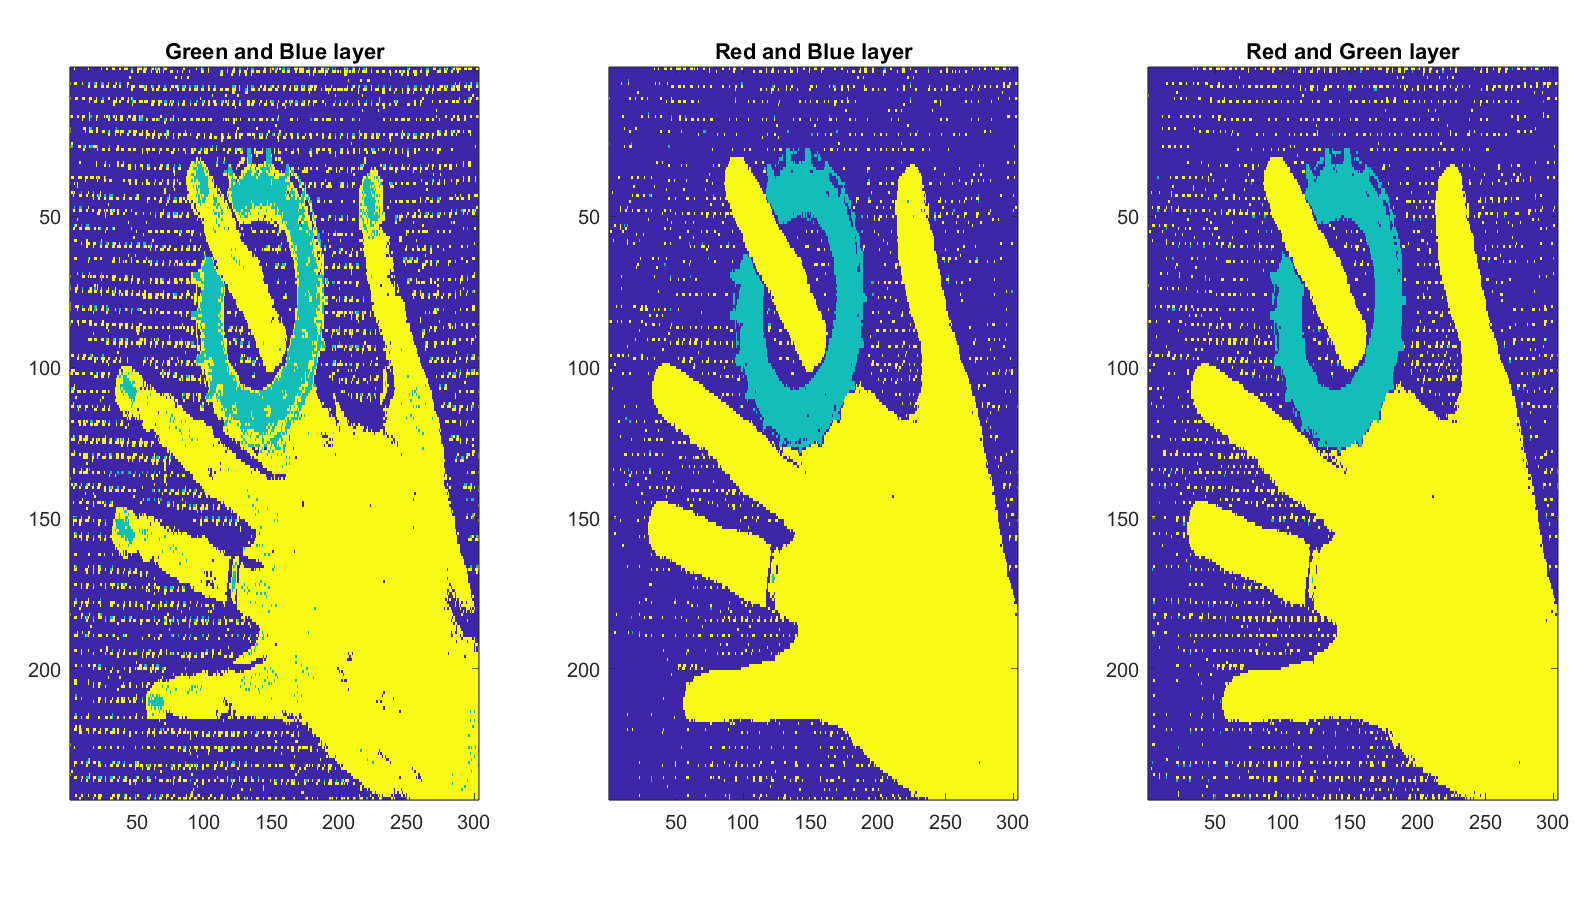
\includegraphics[width =\textwidth]{images/Q4_2b.png}
  \caption{Result of classification of pairs of bands of the image}
  \label{fig:Q4_2}
\end{figure}
Finally, using the full RGB image for classification resulted in a successful outcome, comparable to that of the paired bands. The performance in this case did not show significant improvement over the best-performing pairs. The results of the full RGB classification can be seen in Figure \ref{fig:Q4_3}.
\begin{figure}[htbp!]
  \centering
  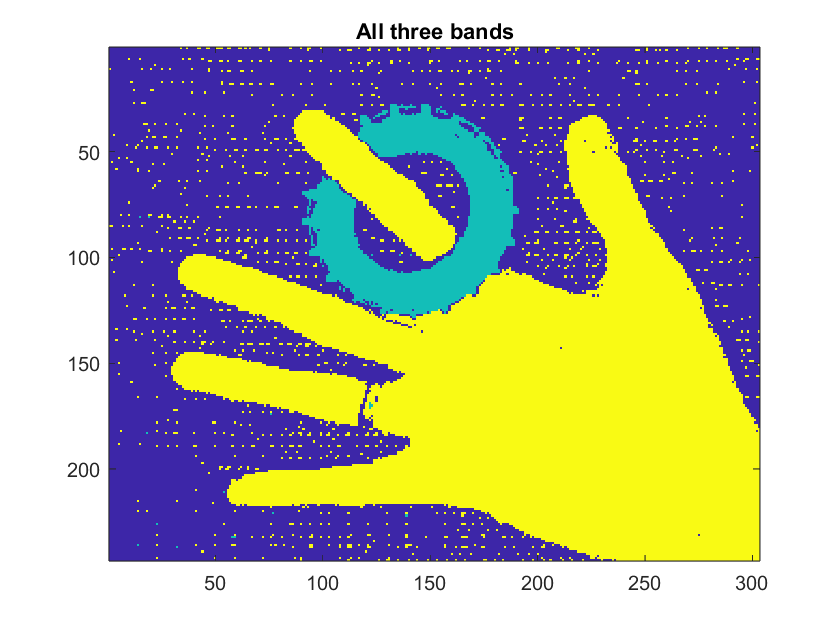
\includegraphics[width = 15cm]{images/Q4_3b.png}
  \caption{Result of classification of pairs of bands of the image}
  \label{fig:Q4_3}
\end{figure}

\section{Classification of multispectral data}
\textbf{\emph{Question 5.}}
% Which bands are you using for your classification? What classifier are you using?
% Which classes are possible to separate in a good way? Illustrate with images and scatterplots. Show images from your classification result and compare with classification using all bands. Discuss your results
Four classes were selected for the satellite image analysis: forest, water, urban areas, and agricultural areas. Corresponding training areas for these classes were identified, as shown in Figure \ref{fig:Q5_res}. Following a comparison of different classifiers, the linear classifier was determined to provide the best results and was used for the final classification.

Several classifications were performed to identify the optimal combination of spectral bands. It was found that the combination [2, 4, 5, 6, 7] produced results identical to using all available bands, which yielded the best classification accuracy. However, the classification faced challenges in distinguishing agricultural areas from urban areas, as evidenced by the presence of several red dots (urban areas) within the light blue regions (agricultural areas) in the figure. Additionally, parts of the forest were misclassified as urban areas. On the other hand, water was the easiest class to identify accurately.

This conclusion is further supported by the scatterplots of different spectral band combinations, shown in Figure \ref{fig:Q5_scatter}. The left scatterplot demonstrated the best separation between classes. Nevertheless, apart from the water class, the scatterplots indicate significant overlap and difficulty in separating the other classes.
\begin{figure}[h!]
  \centering
  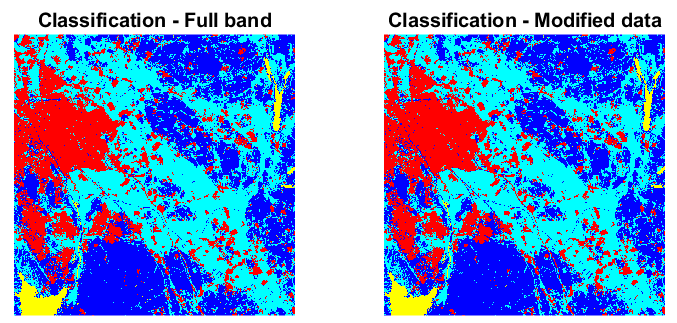
\includegraphics[width = 15cm]{images/Q5_result.png}
  \caption{Result of classification of an satillate picture, the left figure used all the seven bands and the right figure removed band 1 \& 3.}
  \label{fig:Q5_res}
\end{figure}

\begin{figure}[h!]
  \centering
  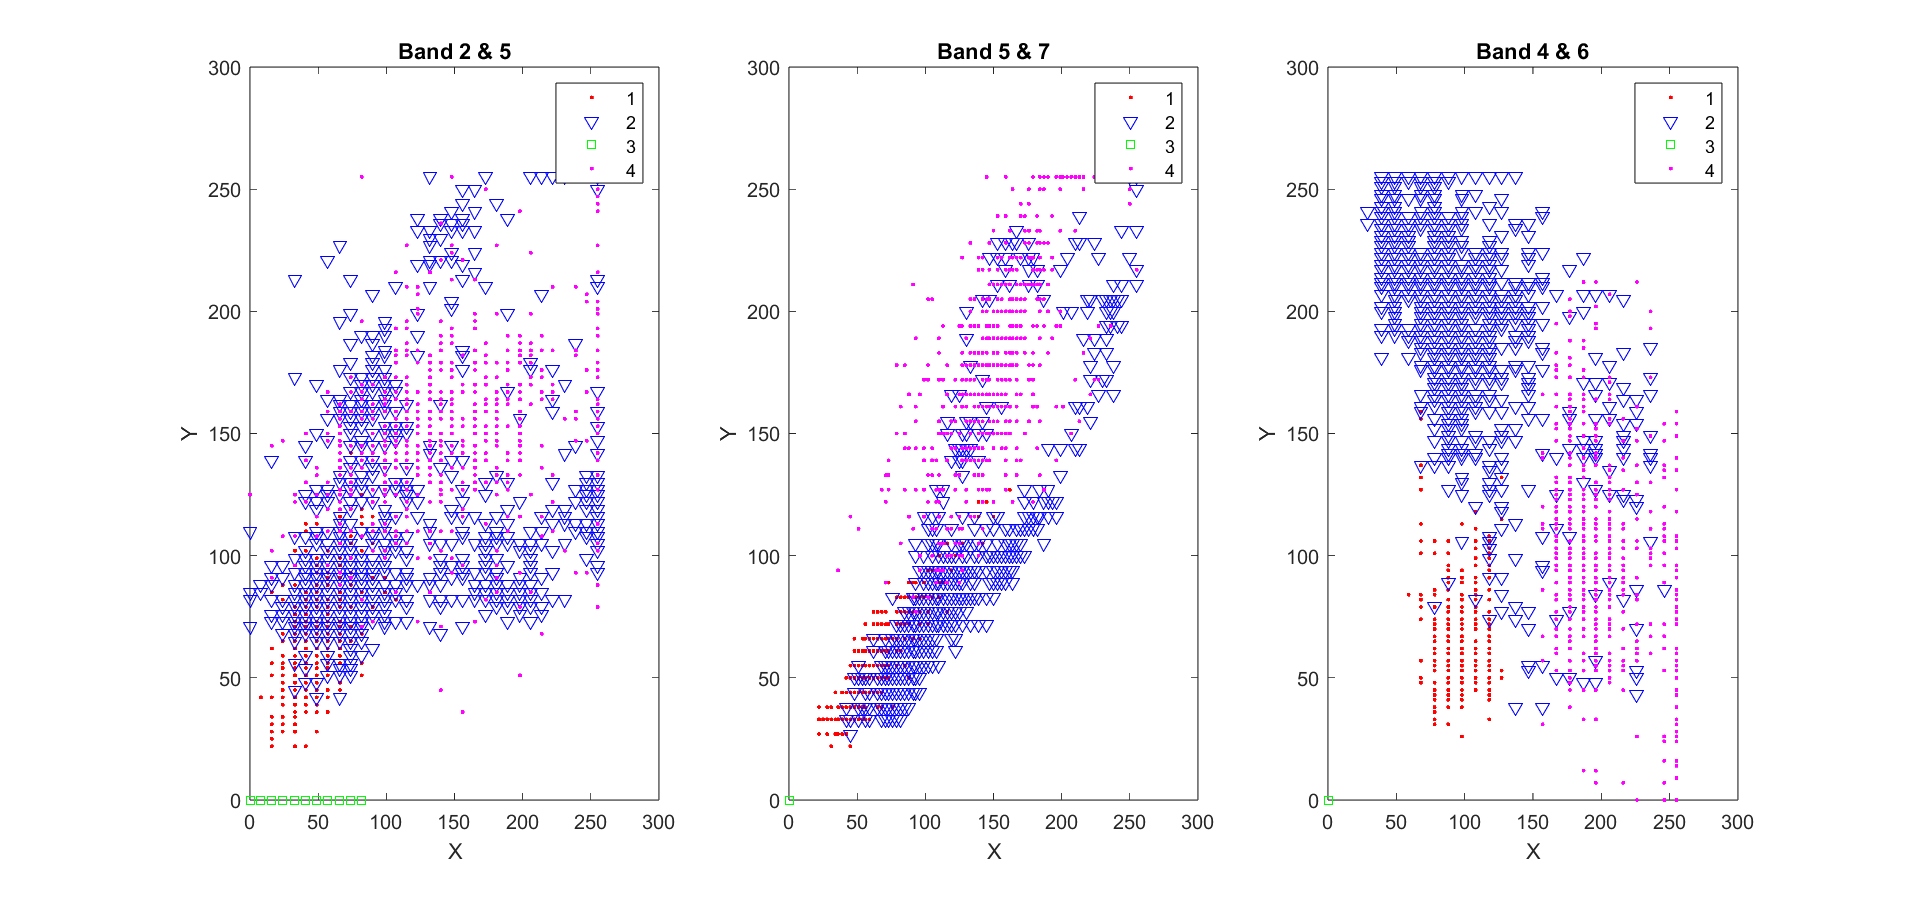
\includegraphics[width = 15cm]{images/Q5_scatter.png}
  \caption{Scatterplot for different combinations of band. 1. Forest, 2. Argicultral area, 3. Water, 4. Urban area. }
  \label{fig:Q5_scatter}
\end{figure}

\textbf{\emph{Question 6.}}
% Is there any reason not to include all bands if they are not needed to separate the classes?
Reducing the number of bands decreases the computational cost; however, excluding bands also eliminates data, which may reduce the robustness and flexibility of the classifier. Therefore, if the improvement in computational efficiency achieved by removing bands is not significant, this step may not be necessary.
\section{Texture-based Classification}
\textbf{\emph{Question 7.}}
% Which ”offset” value did you use for the co-occurrence matrix? Plot uniformity and entropy for all the objects. You should have a plot similar to Figure 3. Using entropy and uniformity, say which objects are outliers and should be removed from the sequence. Why?
The co-occurrence matrix was calculated with the offset [0, 1].


\end{document}

